\subsection{Ordenamiento de Arreglos}
Como podemos ver en ambos graficos (ver Figuras 1 y 2), MergeSort con su complejidad teorica de $O(n \log n)$ en todos los casos tiene un tiempo constante debido a su estrategia de dividir y conquistar, ademas en el grafico de barras se puede ver que sin importar como venga el arreglo tiene un tiempo promedio con respecto a los demas. 

QuickSort tiene un caso promedio de $O(n \log n)$, pero su analisis del peor caso cae a $O(n^2)$ cosa que se demuestra en los graficos: teniendo una demora baja en comparacion a los demas, esta se ve reducida enormemente debido a la distribucion de los arreglos, ya que su pivote queda desbalanceado. 

PatienceSort su complejidad teorica si es que se optimiza bien puede llegar a ser de $O(n \log n)$, pero debido a que en el codigo que use viene con implementacion de codigos dinamicos y una funcion \texttt{v.erase()} que desplaza la memoria en cada extraccion, lleva a este algoritmo a una complejidad ineficiente de $O(n^2)$.

\begin{figure}[H]
    \centering
    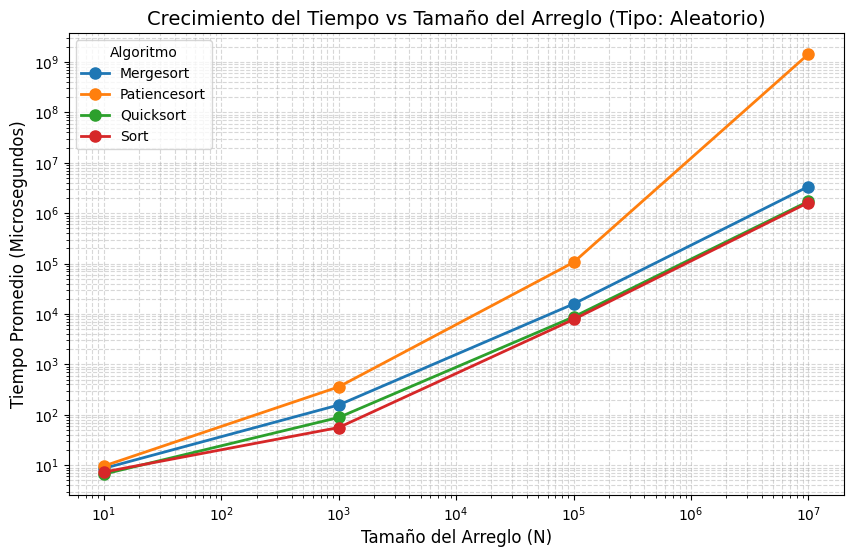
\includegraphics[width=0.8\textwidth]{../code/sorting/data/plots/sorting_tiempo_vs_n.png}
    \caption{Crecimiento del tiempo segun tamaño N.}
\end{figure}

\begin{figure}[H]
    \centering
    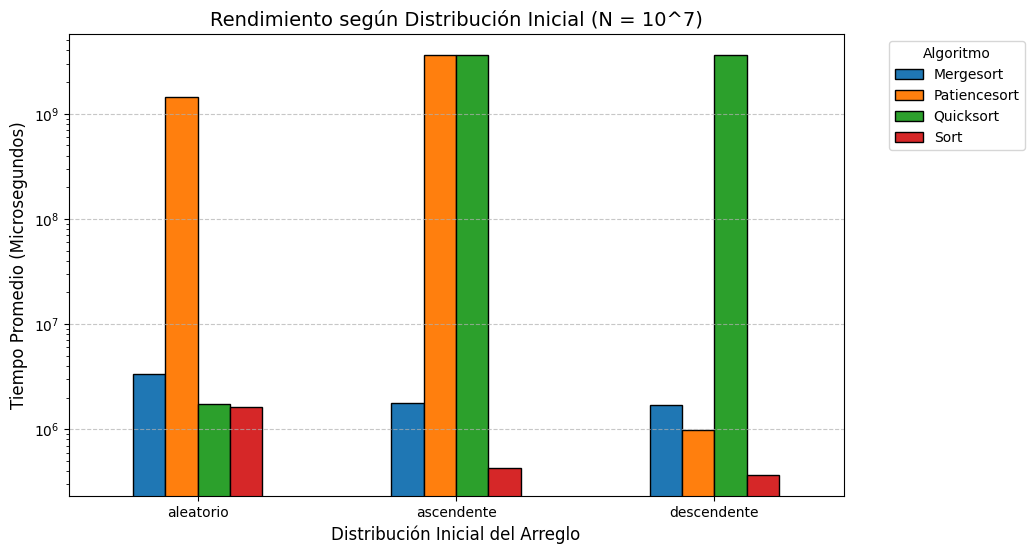
\includegraphics[width=0.8\textwidth]{../code/sorting/data/plots/sorting_comparacion_tipos.png}
    \caption{Rendimiento de ordenamiento segun distribucion.}
\end{figure}

\subsection{Multiplicacion de Matrices}
Por otro lado los algoritmos de multiplicacion de matrices cuadradas (ver Figuras 3 y 4) como el algoritmo Naive que tiene una complejidad teorica de $O(n^3)$ ya que tiene 3 ciclos anidados de tamaño n se demuestra en los graficos de tiempo ya que estos van subiendo a medida que se va agrandando la matriz. 

Por ultimo el algoritmo de Strassen que tiene una complejidad asintotica de $O(n^{2.81})$ pero debido a como se implementa en el codigo que use, que hace muchas sumas de matrices y llamadas recursivas, hace que este suba su tiempo viendose mas lento en el grafico de tiempo en comparacion al Naive.

\begin{figure}[H]
    \centering
    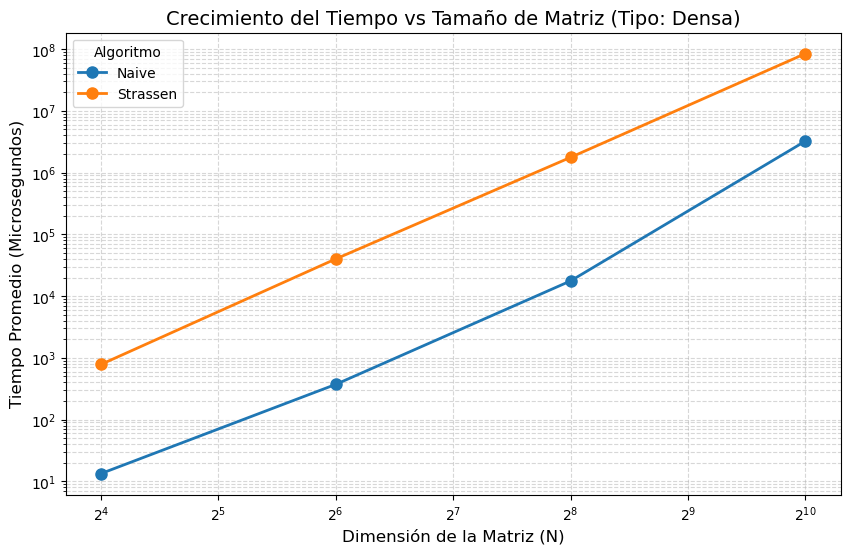
\includegraphics[width=0.8\textwidth]{../code/matrix_multiplication/data/plots/matriz_tiempo_vs_n.png}
    \caption{Crecimiento del tiempo en matrices densas.}
\end{figure}

\begin{figure}[H]
    \centering
    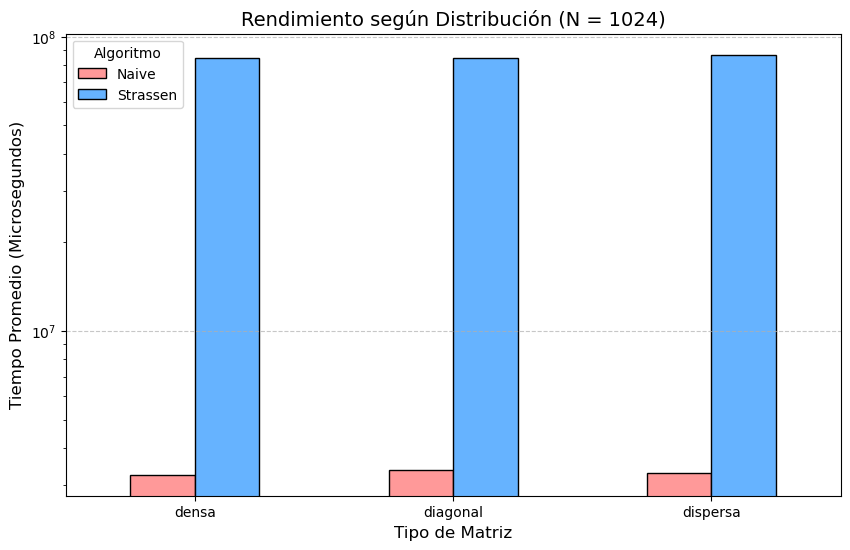
\includegraphics[width=0.8\textwidth]{../code/matrix_multiplication/data/plots/matriz_comparacion_tipos.png}
    \caption{Rendimiento en matrices segun tipo.}
\end{figure}